\documentclass[tikz,border=10pt]{standalone}
\usepackage{amsmath}
\usetikzlibrary{angles,quotes}
\begin{document}
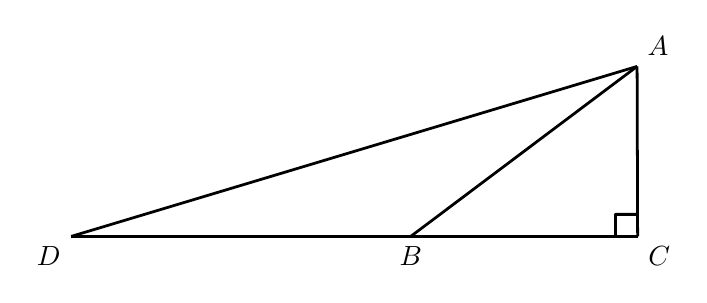
\begin{tikzpicture}[line width=1.0pt, line join=round]
\coordinate (A) at (3.602,1.084);
\coordinate (B) at (0.727,-1.075);
\coordinate (C) at (3.609,-1.075);
\coordinate (D) at (-3.585,-1.075);



\draw (D) -- (A);
\draw (A) -- (B);
\draw (D) -- (B) -- (C);
\draw (A) -- (C);

\draw pic[draw, angle radius=0.280cm] {right angle=A--C--D};

\node[above right, font=\fontsize{10}{12}\selectfont] at (A) {$A$};
\node[below left, font=\fontsize{10}{12}\selectfont] at (D) {$D$};
\node[below, font=\fontsize{10}{12}\selectfont] at (B) {$B$};
\node[below right, font=\fontsize{10}{12}\selectfont] at (C) {$C$};
\end{tikzpicture}
\end{document}